\section{peo\-Pop\-Eval$<$ EOT $>$ Class Template Reference}
\label{classpeo_pop_eval}\index{peoPopEval@{peoPopEval}}
The {\bf {\bf peo\-Pop\-Eval}{\rm (p.\,\pageref{classpeo_pop_eval})}} class provides the interface for constructing Paradis\-EO specific evaluation functors.  


{\tt \#include $<$peo\-Pop\-Eval.h$>$}

Inheritance diagram for peo\-Pop\-Eval$<$ EOT $>$::\begin{figure}[H]
\begin{center}
\leavevmode
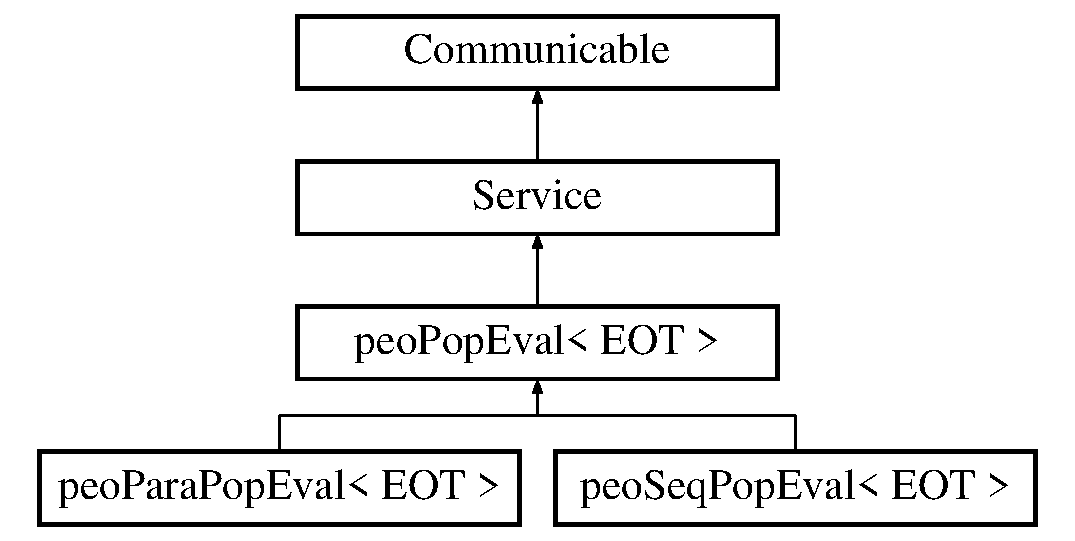
\includegraphics[height=4cm]{classpeo_pop_eval}
\end{center}
\end{figure}
\subsection*{Public Member Functions}
\begin{CompactItemize}
\item 
virtual void {\bf operator()} (eo\-Pop$<$ EOT $>$ \&\_\-\_\-pop)=0\label{classpeo_pop_eval_2f208067a5e39c3b26c1234050a41e8f}

\begin{CompactList}\small\item\em Interface function providing the signature for constructing an evaluation functor. \item\end{CompactList}\end{CompactItemize}


\subsection{Detailed Description}
\subsubsection*{template$<$class EOT$>$ class peo\-Pop\-Eval$<$ EOT $>$}

The {\bf {\bf peo\-Pop\-Eval}{\rm (p.\,\pageref{classpeo_pop_eval})}} class provides the interface for constructing Paradis\-EO specific evaluation functors. 

The derived classes may be used as wrappers for {\bf EO}-derived evaluation functors. In order to have an example, please refer to the implementation of the {\bf {\bf peo\-Seq\-Pop\-Eval}{\rm (p.\,\pageref{classpeo_seq_pop_eval})}} and {\bf {\bf peo\-Para\-Pop\-Eval}{\rm (p.\,\pageref{classpeo_para_pop_eval})}} classes. 



Definition at line 34 of file peo\-Pop\-Eval.h.

The documentation for this class was generated from the following file:\begin{CompactItemize}
\item 
peo\-Pop\-Eval.h\end{CompactItemize}
